\documentclass[11pt,a4paper]{article}
\usepackage{fontspec}
\setmainfont{Noto Sans CJK KR}
\usepackage{amsmath,amssymb,bm}
\usepackage{booktabs}
\usepackage{graphicx}
\usepackage{geometry}
\geometry{margin=2.3cm}
\usepackage[hidelinks]{hyperref}
\usepackage{caption}
\captionsetup{font=small}
\usepackage{enumitem}
\usepackage{mdframed}

\newcommand{\cL}{\mathcal{L}}

\title{\textbf{L4 리스크 카드의 3단 해상도 릴리스 설계}\\[4pt]
\large Master / C80 / C70 세트 생성을 위한 반복 병합 절차와 임계값 선택}
\author{RAI Risk Taxonomy 2.0 --- v2.19 통합 라운드 기술 보고서}
\date{2026년 8월 6일}

\begin{document}
\maketitle

\begin{abstract}
본 보고서는 RAI Risk Taxonomy 2.0의 L4 리스크 카드 집합을 서로 다른 세 해상도로 릴리스하기 위한 통합 절차를 기술한다. 목표는 군집 분석 뷰의 생성이 아니라, 각 해상도마다 실제 카드가 존재하고 카드 수가 감소하는 세 개의 독립 릴리스 세트(Master, C80, C70)를 만드는 것이다. 본 보고서는 (i) Master 세트를 1{,}652장으로 확정하고 그 실효 임계값 $\tau_{\mathrm{eff}}=0.945$를 산출하며, (ii) 통합 절차를 반복 병합 루프로 형식화하고 연결 규칙(linkage) 네 종을 실증 비교하며, (iii) $\tau \in [0.60, 0.99]$ 전 구간 스윕 결과를 보고하고, (iv) 명명가능성 검정을 병합 게이트로 도입할 것을 제안한다. 주요 실증 결과는 두 가지다. 첫째, $\tau=0.95$부터 $0.84$까지 카드 수는 1{,}660에서 1{,}607로 3.2\%만 감소하며 실질적 감축은 $\tau<0.82$에서 시작한다. 둘째, 중심 연결(centroid)과 단일 연결(single)은 $\tau=0.70$에서 각각 최대 군집 1{,}191장과 1{,}514장으로 붕괴하므로, 목표 해상도에서 사용 가능한 연결 규칙은 완전 연결(complete)뿐이다. 본 보고서는 설계와 실증까지만 다루며, 임베딩 재생성 이후의 실제 세트 생성은 수행하지 않았다.
\end{abstract}

\section{목적과 범위}

\subsection{요구사항}

세 개의 릴리스 세트를 만든다.

\begin{itemize}[leftmargin=1.6em,itemsep=2pt]
  \item \textbf{Master} --- 현행 세트. 적용된 임계값을 기록한다.
  \item \textbf{C80} --- $\tau=0.80$ 수준으로 압축한 세트.
  \item \textbf{C70} --- $\tau=0.70$ 수준으로 압축한 세트.
\end{itemize}

핵심 요구는 세 세트가 각각 \emph{완결된 카드 집합}이라는 점이다. 즉 C70은 ``1{,}652장을 847개 군집으로 묶어 본 뷰''가 아니라, 847장의 카드가 각자 고유 ID, 명칭, 정의, 참고문헌, 부모 L3를 갖는 릴리스여야 한다. 카드 수 자체의 감축이 목적이다.

\subsection{본 보고서가 다루지 않는 것}

임베딩 재생성, 클러스터링 실행, 병합 카드 명명, 세트 산출물 생성은 수행하지 않았다. 본 보고서의 모든 수치는 v2.18.0-rc 기준 기존 정본 임베딩에서 산출한 것이며, 제\ref{sec:limits}절에서 그 한계를 명시한다.

\section{Master 세트의 확정}

\subsection{구성}

v2.18.0-rc 릴리스는 총 1{,}711장(활성 1{,}660, 은퇴 51)으로 구성된다. 여기에 v2.19 통합 라운드의 두 가지 확정 사항을 적용하여 Master를 정의한다.

\begin{enumerate}[leftmargin=1.6em,itemsep=2pt]
  \item \textbf{승인 병합 8건.} 2인 검수 합의(\texttt{two\_reviewer\_consensus\_20260806})로 확정된 8건의 병합. 원 카드 16장을 은퇴시키고 신규 ID \texttt{RAI4-1727}--\texttt{1734}를 부여한다.
  \item \textbf{라벨 교정 204장.} 도메인 용어 오역 및 기계번역 직역 170장(한글 라벨), 서술문형 라벨의 명사구 재작명 34장(한/영 라벨).
\end{enumerate}

결과는 \textbf{활성 1{,}652장}, 은퇴 누적 67장이다. 사용 중인 L3 노드는 56개로 변동이 없다.

\subsection{실효 임계값 $\tau_{\mathrm{eff}}$}

Master에 명시적으로 적용된 임계값은 병합 판정에 사용한 운용값 $\tau_{\mathrm{gov}}=0.88$이다. 그러나 이 값은 심의 대상을 고르는 기준이었을 뿐, 세트의 실제 해상도를 규정하지 않는다. 세트의 해상도를 규정하는 값은 다음과 같이 정의한다.

\begin{equation}
\tau_{\mathrm{eff}} \;=\; \max_{i \neq j} \; \cos(\mathbf{e}_i, \mathbf{e}_j) \;+\; \epsilon,
\end{equation}

즉 이 값 이상에서는 어떤 두 카드도 병합되지 않는 최소 임계값이다. 실측 결과 활성 카드 쌍의 최대 코사인 유사도는 $0.9437$이며, 따라서 $\tau_{\mathrm{eff}} = 0.945$이다.

주목할 점은 이 최댓값을 만드는 쌍이 \texttt{RAI4-0659}--\texttt{RAI4-0892}라는 사실이다. 이 쌍은 전문가 심의에서 \emph{병합 금지}로 판정된 임베딩 위양성 쌍이다. 즉 임베딩 공간에서 가장 가까운 두 카드가 의미적으로는 합쳐서는 안 되는 쌍이며, 이는 임계값 단독 판정의 한계를 보여주는 직접 증거다.

유사도 분포의 상위 꼬리는 다음과 같다. $\cos \geq 0.88$인 쌍 12개, $\cos \geq 0.84$인 쌍 62개, $\cos \geq 0.80$인 쌍 342개다. 전체 쌍 수가 약 137만 개임을 고려하면 상위 꼬리는 매우 얇다.

\section{통합 절차의 형식화}

\subsection{반복 병합 루프}

통합은 응집형 계층 병합(agglomerative merging)으로 수행한다. 절차는 다음과 같다.

\begin{mdframed}[linewidth=0.5pt,innertopmargin=6pt,innerbottommargin=6pt]
\textbf{Procedure} \textsc{IterativeMerge}$(\{\mathbf{e}_i\}, \tau)$
\begin{enumerate}[leftmargin=2.0em,itemsep=1pt]
  \item 각 카드를 크기 1의 단위 $\cL_i \leftarrow \{r_i\}$로 초기화한다.
  \item 살아있는 모든 단위 쌍 $(\cL_a, \cL_b)$에 대해 단위 간 유사도 $\sigma(\cL_a, \cL_b)$를 계산한다.
  \item $\sigma$가 최대인 쌍을 선택한다. 그 값이 $\tau$ 미만이면 종료한다.
  \item 선택된 쌍을 하나의 단위로 통합하고, 통합체를 포함하여 2단계로 돌아간다.
\end{enumerate}
\end{mdframed}

이 루프는 매 단계에서 가장 유사한 쌍을 통합하고 통합체를 포함해 재계산한다. 덴드로그램은 이 반복 과정 전체를 기록한 트리이며, $\tau$로 절단한다는 것은 유사도가 $\tau$ 아래로 떨어지는 시점에서 루프를 정지시키는 것과 동치이다.

\subsection{연결 규칙 $\sigma$의 선택}

절차의 유일한 자유도는 통합체의 유사도를 어떻게 정의하는가, 즉 $\sigma$의 선택이다. 네 가지 후보가 있다.

\begin{table}[h]
\centering
\small
\begin{tabular}{@{}lll@{}}
\toprule
규칙 & $\sigma(\cL_a, \cL_b)$ & 성격 \\
\midrule
Complete & $\min_{i \in \cL_a, j \in \cL_b} \cos(\mathbf{e}_i, \mathbf{e}_j)$ & 군집 내 모든 쌍이 $\tau$ 이상임을 보장 \\
Average  & $\frac{1}{|\cL_a||\cL_b|}\sum_{i,j} \cos(\mathbf{e}_i, \mathbf{e}_j)$ & 평균적 응집 \\
Centroid & $\cos(\bar{\mathbf{e}}_a, \bar{\mathbf{e}}_b)$ & 통합체를 평균 벡터 한 점으로 재표현 \\
Single   & $\max_{i \in \cL_a, j \in \cL_b} \cos(\mathbf{e}_i, \mathbf{e}_j)$ & 연쇄 병합 \\
\bottomrule
\end{tabular}
\caption{연결 규칙 후보. Centroid는 ``통합된 것을 포함해 전체 유사도를 재계산''이라는 직관적 서술에 가장 가깝다.}
\end{table}

다섯 번째 대안으로 \textbf{재임베딩 방식}이 있다. 통합 단위마다 새 명칭과 정의를 실제로 작성하고 그 텍스트를 다시 임베딩하여 다음 라운드의 유사도를 계산하는 것이다. 의미론적으로는 가장 정확하지만, 매 병합 단계마다 명명이 필요하므로 수백 회 반복 시 비용이 지배적이다.

\subsection{연결 규칙의 실증 비교}

네 규칙을 동일 임베딩과 동일 $\tau$에서 실행한 결과는 표\,\ref{tab:linkage}와 같다.

\begin{table}[h]
\centering
\small
\begin{tabular}{@{}llrrrrr@{}}
\toprule
$\tau$ & 규칙 & 카드 수 & 다중 군집 & 최대 군집 & 평균 군집 크기 & L3 교차 \\
\midrule
0.80 & complete & 1{,}458 & 188 & 4 & 2.07 & 100 \\
0.80 & average  & 1{,}445 & 184 & 5 & 2.17 & 102 \\
0.80 & centroid & 1{,}383 & 161 & 12 & 2.72 & 97 \\
0.80 & single   & 1{,}360 & 150 & 44 & 3.00 & 93 \\
\midrule
0.70 & complete & 844 & 510 & 8 & 2.60 & 341 \\
0.70 & average  & 702 & 384 & 21 & 3.49 & 270 \\
0.70 & centroid & 354 & 77 & \textbf{1{,}191} & 17.96 & 49 \\
0.70 & single   & 128 & 18 & \textbf{1{,}514} & 86.11 & 13 \\
\bottomrule
\end{tabular}
\caption{연결 규칙별 실측(활성 1{,}660장, BGE-M3 정본 임베딩). $\tau=0.70$에서 centroid와 single은 붕괴한다.}
\label{tab:linkage}
\end{table}

결과는 명확하다. $\tau=0.80$에서는 네 규칙이 대체로 비슷한 규모를 산출하지만, $\tau=0.70$에서 centroid는 최대 군집이 1{,}191장, single은 1{,}514장으로 붕괴한다. 전체 카드의 70--91\%가 단 하나의 단위로 합쳐지는 것이다. 이는 평균 벡터가 병합될수록 공간의 중심으로 이동하여 남은 모든 단위와 가까워지는 중심 이동(centroid drift) 현상이다.

따라서 \textbf{목표 해상도에서 사용 가능한 연결 규칙은 complete뿐이다.} Average는 $\tau=0.70$에서 최대 군집 21장으로 붕괴하지는 않으나, 21장을 포괄하는 단일 카드 명칭을 작성하는 것은 현실적으로 불가능하다.

\section{$\tau$ 스윕 실측}

$\tau \in [0.60, 0.99]$ 구간을 $0.01$ 간격으로 complete linkage로 스윕한 결과를 표\,\ref{tab:sweep}과 그림\,\ref{fig:tau}에 제시한다.

\begin{table}[h]
\centering
\small
\begin{tabular}{@{}rrrrrrrr@{}}
\toprule
$\tau$ & 카드 수 & 감축 & 감축률 & 다중 군집 & 단일 카드 & L3 교차 & L1 교차 \\
\midrule
0.945 & 1{,}660 & 0 & 0.0\% & 0 & 1{,}660 & 0 & 0 \\
0.90 & 1{,}653 & 7 & 0.4\% & 7 & 1{,}646 & 3 & 1 \\
0.88 & 1{,}648 & 12 & 0.7\% & 12 & 1{,}636 & 5 & 1 \\
0.84 & 1{,}607 & 53 & 3.2\% & 53 & 1{,}554 & 27 & 2 \\
0.82 & 1{,}545 & 115 & 6.9\% & 109 & 1{,}436 & 54 & 11 \\
\textbf{0.80} & \textbf{1{,}458} & 202 & 12.2\% & 188 & 1{,}270 & 100 & 25 \\
0.76 & 1{,}233 & 427 & 25.7\% & 346 & 887 & 205 & 64 \\
0.73 & 1{,}036 & 624 & 37.6\% & 458 & 578 & 283 & 95 \\
\textbf{0.70} & \textbf{844} & 816 & 49.2\% & 510 & 334 & 341 & 115 \\
0.65 & 567 & 1{,}093 & 65.8\% & 453 & 114 & 351 & 134 \\
0.60 & 370 & 1{,}290 & 77.7\% & 342 & 28 & 297 & 143 \\
\bottomrule
\end{tabular}
\caption{$\tau$ 스윕 (complete linkage, 제약 없음). ``L3 교차''는 구성원이 둘 이상의 L3에 걸친 군집 수, ``L1 교차''는 최상위 분기에 걸친 군집 수.}
\label{tab:sweep}
\end{table}

\begin{figure}[h]
\centering
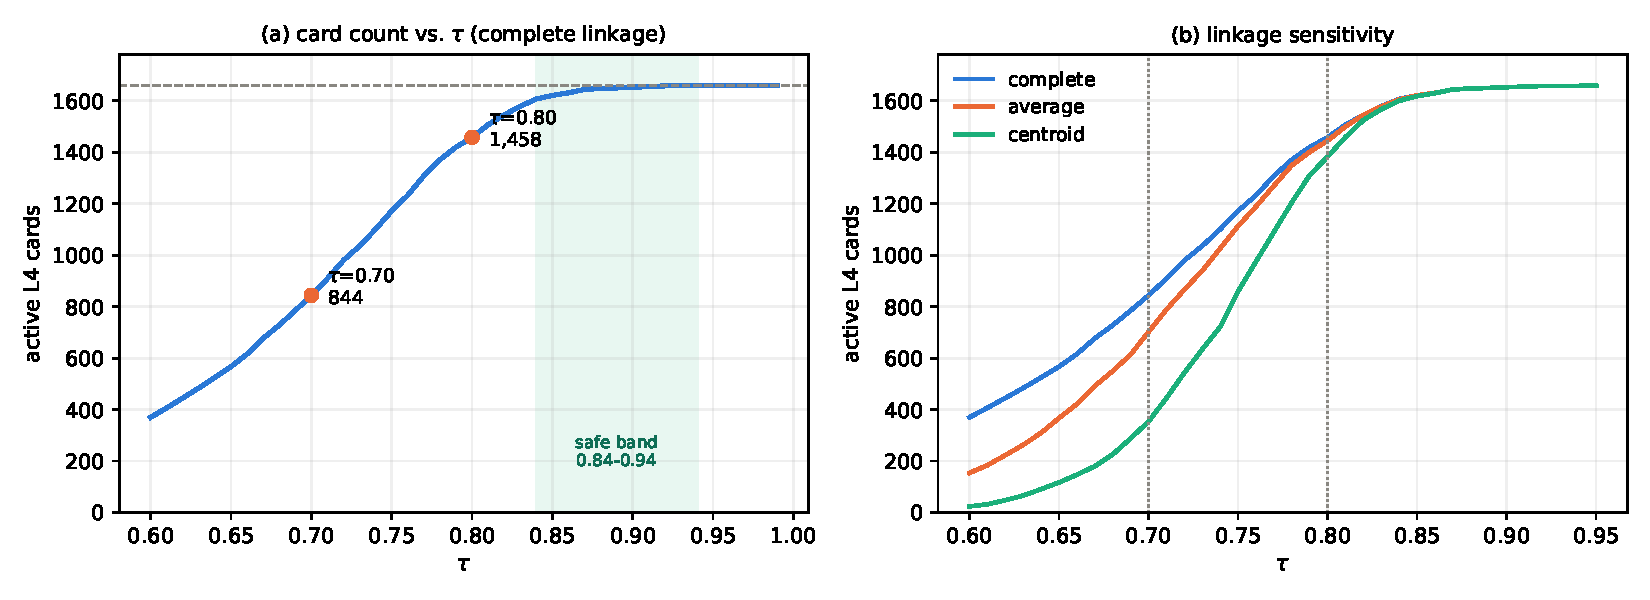
\includegraphics[width=\textwidth]{fig_tau_tiers.pdf}
\caption{(a) $\tau$에 따른 카드 수 곡선과 안전 운용대. (b) 연결 규칙별 민감도. centroid는 $\tau<0.75$에서 급격히 붕괴한다.}
\label{fig:tau}
\end{figure}

곡선의 형태에서 세 가지가 관찰된다.

첫째, \textbf{$\tau=0.945$에서 $0.84$까지 구간은 사실상 평평하다.} 감축은 53장(3.2\%)에 불과하다. 이는 임베딩 공간에서 진짜 근접 쌍이 극히 희소함을 뜻하며, $\tau_{\mathrm{eff}}$ 부근에서의 병합이 곧 ``실질 중복 제거''임을 시사한다.

둘째, \textbf{실질 감축은 $\tau<0.82$에서 시작한다.} 0.82에서 6.9\%, 0.80에서 12.2\%, 0.76에서 25.7\%로 가속한다.

셋째, \textbf{$\tau=0.80$ 세트는 Master와 88\% 동일하다.} 1{,}458장 중 1{,}270장이 병합되지 않은 원 카드이며, 신규 생성되는 통합 카드는 188장뿐이다. 세 세트를 뚜렷이 구분되는 해상도로 제시하려는 목적에 비추어 보면, C80은 Master의 변형에 가깝다는 지적이 가능하다.

\section{cannot-link 제약}

\subsection{문제}

전문가 심의에서 \emph{병합 금지}로 확정된 4쌍이 있다.

\begin{center}
\small
\texttt{RAI4-0228}--\texttt{0229} \quad \texttt{RAI4-0659}--\texttt{0892} \quad \texttt{RAI4-0863}--\texttt{0870} \quad \texttt{RAI4-0682}--\texttt{0691}
\end{center}

이들의 코사인 유사도는 각각 0.944, 0.905, 0.883 수준으로 임베딩 위양성이다. 제약 없이 $\tau \leq 0.88$로 절단하면 \textbf{4쌍 전부가 병합된다.} 즉 목표 해상도 $\tau=0.80$과 $0.70$에서는 전문가가 명시적으로 부정한 병합이 자동으로 발생한다.

\subsection{해결}

제약 클러스터링으로 강제한다. 병합 금지 쌍 $(i,j)$의 거리를 $d_{ij} \leftarrow \infty$로 설정한 뒤 complete linkage를 수행하면, complete의 정의상 두 카드를 포함하는 어떤 두 단위도 거리 $\infty$를 가지므로 결코 병합되지 않는다. 이 성질은 complete linkage에만 성립한다.

제약 적용 시 카드 수 변화는 미미하다. $\tau=0.80$에서 1{,}458 $\rightarrow$ 1{,}462, $\tau=0.70$에서 844 $\rightarrow$ 847이며, 위반 건수는 모두 0이 된다. 반면 centroid와 single에 동일한 제약을 적용하면 위반이 각각 1건, 3건 잔존하는데, 평균 벡터나 최댓값 연결에서는 $\infty$ 거리가 전파되지 않기 때문이다. 이는 complete linkage를 선택해야 할 두 번째 독립적 근거다.

\section{명명가능성 검정}

\subsection{동기}

선행 분석에서 golden set(승인 병합 8쌍을 양성, 병합 금지 4쌍을 음성으로 사용)에 대한 $\tau$별 precision/recall 분석 결과, 과소병합 임계선은 $\tau>0.84$, 과대병합 임계선은 $\tau<0.94$였다. 즉 안전 운용대는 $0.84 \leq \tau < 0.94$이다.

목표 해상도 $\tau=0.80$과 $0.70$은 \textbf{이 구간 밖, 즉 과대병합 구간에 있다.} 따라서 $\tau$로 절단한 결과를 그대로 카드로 승격하는 것은 데이터가 지지하지 않는다.

\subsection{제안}

임계값 대신 인간 판정을 게이트로 사용한다. 각 통합 단위에 대해 검수자가 다음을 시도한다.

\begin{quote}
\textit{구성원 전부를 포괄하는 진짜 상위어를, 명사구로, 영문 12단어 이내로 작성할 수 있는가?}
\end{quote}

작성 가능하면 병합을 승인하고 그 명칭을 신규 카드에 부여한다. 작성이 불가능하거나 결과가 나열식이 되면(예: ``프롬프트 주입 및 데이터 오염 및 모델 추출'') 병합을 기각하고 해당 단위는 분리 상태로 유지한다.

이 검정은 두 가지 기능을 한다. 첫째, 통합 카드의 명칭을 생산한다. 둘째, 명칭을 쓸 수 없다는 사실 자체가 그 군집이 의미적으로 하나가 아니라는 증거이므로 과대병합 필터로 작동한다. 명명 산출물과 병합 판정이 동일한 행위에서 나오는 것이 이 설계의 요점이다.

명명 부담은 $\tau=0.80$에서 188건, $\tau=0.70$에서 510건이다. 선행 라운드에서 204장 라벨 교정을 11개 배치 병렬 검수로 처리한 전례가 있으므로 절차적으로는 가능하나, C70은 규모가 2.5배이며 군집당 구성원 수도 평균 2.6장으로 늘어난다.

\section{병합 카드의 속성 집계}

통합 단위 $\cL$로부터 신규 카드를 생성할 때의 규칙을 사전 확정한다.

\begin{table}[h]
\centering
\small
\begin{tabular}{@{}ll@{}}
\toprule
속성 & 규칙 \\
\midrule
\texttt{l4\_id} & 신규 연번 부여(현행 최대 \texttt{RAI4-1734} 이후) \\
\texttt{label\_ko/en} & 명명가능성 검정에서 확정된 상위어 \\
\texttt{definition\_ko/en} & 상위 개념 정의 + 구성원 사례 열거 \\
\texttt{severity\_1to5} & $\max_{i \in \cL} s_i$ (보수적) \\
\texttt{probability\_0to1} & $\max_{i \in \cL} p_i$ (합집합 사건의 하한) \\
\texttt{references} & 구성원 참고문헌의 합집합(중복 제거) \\
\texttt{three\_h\_one\_r} & 구성원 라벨의 합집합 \\
\texttt{primary\_l3\_id} & 동일 L3면 승계, 교차 시 심의(제\ref{sec:limits}절) \\
\texttt{merged\_source\_l4\_ids} & 구성원 원 ID 전체(계보) \\
\bottomrule
\end{tabular}
\caption{병합 카드 속성 집계 규칙.}
\end{table}

\texttt{probability}에 최댓값을 쓰는 근거는 병합 카드가 구성원 사건의 합집합을 표상하므로 $P(\bigcup_i A_i) \geq \max_i P(A_i)$이기 때문이다. 이는 하한이며 참값은 아니다.

\section{중첩 구조와 ID 매핑}

세 세트를 각각 독립적으로 클러스터링하면 상호 계보가 성립하지 않는다. 대신 동일한 덴드로그램을 서로 다른 지점에서 절단한다. Complete linkage의 단조성에 의해 $\tau$가 낮아질수록 군집은 병합만 되고 분할되지 않으므로 다음이 성립한다.

\begin{equation}
\text{Master} \;\supseteq\; \text{C80} \;\supseteq\; \text{C70}
\end{equation}

즉 모든 C70 카드는 C80 카드들의 합집합이고, 모든 C80 카드는 Master 카드들의 합집합이다. 이로써 세트 간 ID 매핑이 트리로 떨어지며, 외부 인용이 어느 해상도를 참조하든 다른 해상도로 결정론적으로 변환된다.

단, 명명가능성 검정에서 일부 병합이 기각되면 이 성질이 깨질 수 있다. C70에서 승인된 병합의 부분집합이 C80에서 기각되는 경우가 그것이다. 이를 방지하려면 검정을 C80에서 먼저 수행하고, C70은 승인된 C80 카드를 단위로 삼아 진행해야 한다. 즉 절단은 한 번에 하되 검정은 해상도 순으로 누적해야 한다.

\section{한계와 미해결 쟁점}
\label{sec:limits}

\subsection{임베딩 미갱신}

본 보고서의 모든 수치는 v2.18.0-rc 기준 임베딩에서 산출했다. Master 확정 과정에서 204장(12.3\%)의 라벨이 교정되었고, 라벨은 임베딩 텍스트(\texttt{label\_en. definition\_en / label\_ko. definition\_ko})에 포함된다. 따라서 재생성 후 군집 구성과 카드 수는 변동한다. 보고된 1{,}458과 844는 확정치가 아니라 규모 추정치다.

\subsection{목표 해상도가 안전 운용대 밖}

$\tau=0.80$과 $0.70$은 golden set 기반 안전 운용대 $[0.84, 0.94)$ 밖이다. 명명가능성 검정을 게이트로 도입하는 것이 본 보고서의 대응이나, 이는 통계적 보증이 아니라 절차적 보증이다.

\subsection{golden set의 표본 크기}

안전 운용대는 양성 8쌍, 음성 4쌍, 총 12쌍에서 추정되었다. 임계선 $0.84$와 $0.94$는 각각 단일 쌍(코사인 0.844의 도구 오용 쌍, 0.944의 폭력/비폭력 범죄 쌍)에 의해 결정되므로, 표본 하나가 임계선 전체를 좌우한다. 신뢰구간을 제시할 수 없다.

\subsection{L3 교차 병합}

$\tau=0.80$에서 100건, $\tau=0.70$에서 341건의 군집이 둘 이상의 L3에 걸친다. C70의 경우 다중 군집 510개 중 341개(67\%)가 교차 병합이다. 이들 카드의 부모 L3를 결정하는 것은 사실상 L3 체계 재설계에 해당하며, 본 보고서는 절차를 제시하지 않았다. L1 교차도 $\tau=0.70$에서 115건 발생한다.

\subsection{세 세트의 사용자 측 의미}

동일 리스크가 세 세트에서 서로 다른 ID와 명칭으로 존재하게 된다. 외부 인용, 규제 매핑, 기존 논문 참조가 어느 세트를 정본으로 삼는지 명시하지 않으면 혼란이 발생한다. 릴리스 정책 차원의 결정이 필요하다.

\subsection{재임베딩 방식 미검증}

제3.2절의 다섯 번째 대안인 재임베딩 방식은 의미론적으로 가장 타당하나 본 보고서에서 실행하지 않았다. Complete linkage 결과와의 차이가 얼마인지 알 수 없다.

\section{실행 계획}

\begin{enumerate}[leftmargin=1.6em,itemsep=2pt]
  \item Master 1{,}652장 기준 정본 임베딩 재생성(BGE-M3, \texttt{max\_seq\_length}=256, L2 정규화).
  \item cannot-link 제약을 적용한 complete linkage 덴드로그램 1회 생성.
  \item $\tau=0.80$ 절단 $\rightarrow$ C80 후보 군집 $\rightarrow$ 명명가능성 검정 $\rightarrow$ C80 확정.
  \item C80 카드를 단위로 $\tau=0.70$ 절단 $\rightarrow$ C70 후보 군집 $\rightarrow$ 검정 $\rightarrow$ C70 확정.
  \item 세 세트의 \texttt{cards.json}, \texttt{hierarchy.json}, ID 매핑, manifest 생성.
  \item 검증: cannot-link 위반 0건, 중첩 구조 무결성, ID 매핑 왕복 무손실, 카드 수 일치, L3 배정 근거 기록 완전성.
\end{enumerate}

\section{결론}

Master 세트는 1{,}652장, $\tau_{\mathrm{eff}}=0.945$로 확정된다. C80과 C70의 생성 절차는 cannot-link 제약을 적용한 complete linkage 반복 병합과 명명가능성 검정의 결합으로 설계되었다. 연결 규칙 선택에 대해서는 실증적 결론이 명확하다---centroid와 single은 목표 해상도에서 붕괴하며, cannot-link 제약을 보존하지 못하므로 complete linkage가 유일한 선택지다. 반면 목표 해상도 자체가 통계적 안전 운용대 밖이라는 점은 해소되지 않았으며, 명명가능성 검정이라는 절차적 장치에 의존한다. 이 의존이 수용 가능한지가 본 설계의 핵심 판단 지점이다.

\end{document}
